\documentclass{article}
\usepackage{amsmath, amssymb, cite, algorithmic, url, braket}
\usepackage{graphicx}
\usepackage{subfigure}
\usepackage{pythonhighlight}
\usepackage[margin=1.5cm]{geometry}
\usepackage[title]{appendix}
\usepackage{listings}
\usepackage{booktabs}

\graphicspath{{../pic/}}
\lstset{
language=[ANSI]{C},
showtabs=true,
tab=,
tabsize=2,
basicstyle=\ttfamily\footnotesize,%\setstretch{.5},
stringstyle=\color{stringcolour},
showstringspaces=false,
alsoletter={1234567890},
otherkeywords={\%, \}, \{, \&, \|},
keywordstyle=\color{keywordcolour}\bfseries,
upquote=true,
morecomment=[s]{/*}{*/},
commentstyle=\color{commentcolour}\slshape,
literate=*%
{=}{{\literatecolour=}}{1}%
{-}{{\literatecolour-}}{1}%
{+}{{\literatecolour+}}{1}%
{*}{{\literatecolour*}}{1}%
{!}{{\literatecolour!}}{1}%
{[}{{\literatecolour[}}{1}%
{]}{{\literatecolour]}}{1}%
{<}{{\literatecolour<}}{1}%
{>}{{\literatecolour>}}{1}%
% {>>>}{\pythonprompt}{3}%
,%
frame=trbl,
rulecolor=\color{black!40},
backgroundcolor=\color{white},
breakindent=.5\textwidth,frame=single,breaklines=true
}

\begin{document}
\title{DSP Monthly Project 01}
\author{Xu, Minhuan}
\maketitle
\tableofcontents
\begin{abstract}
I will use my Raspberry Pi to launch a server of MJPG-streamer to broadcast the stream captured by the CSI camera and in help of fast reverse proxy to broadcast the live-stream to Public Network.
\end{abstract}

\section{Introduction}
\subsection{Raspberry Pi}
Raspberry Pi is a card micro computer which has almost everything a normal PC has, such as a 1000M Ethernet port, USB 3.0 and 2.0, HDMI output, $3.5 ~ \mathrm{mm}$ earphone port and the most important in my project, the CSI camera module.

\begin{figure}[!h]
	\centering
	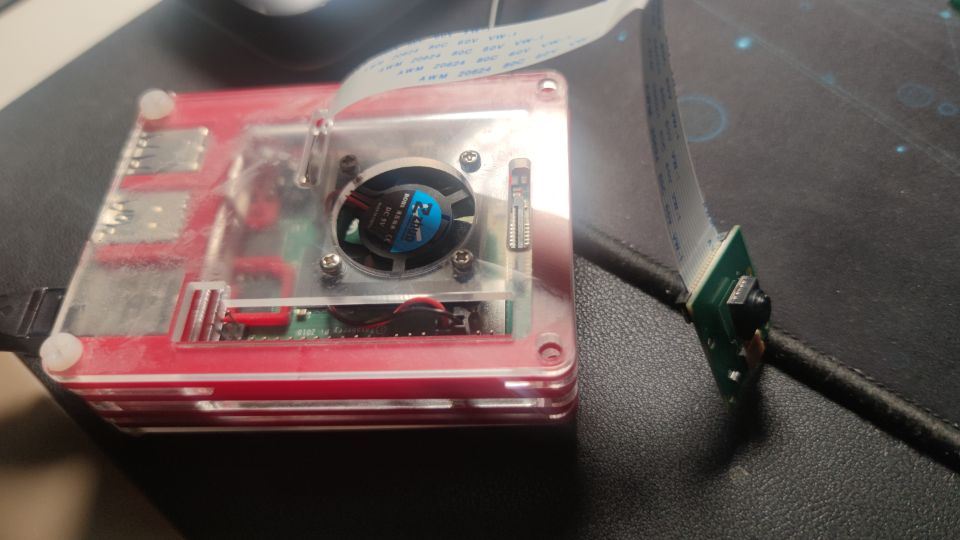
\includegraphics[width=3 in]{../pic/raspi-photo.jpg}
	\caption{My Raspberry Pi}
	\label{fig:raspi-photo}
\end{figure}

\subsection{MJPG-streamer}
MJPG-streamer is a command line application that copies JPEG frames from one or more input plugins to multiple output plugins.  It can be used to stream JPEG files over an IP-based network from a webcam to various types of viewers such as Chrome, Firefox, VLC, and other software capable of receiving MJPG streams. \cite{gh:mjpg-streamer}

\subsection{FRP}
frp is a fast reverse proxy to help you expose a local server behind a NAT or firewall to the Internet.  As of now, it supports TCP and UDP, as well as HTTP and HTTPS protocols, where requests can be forwarded to internal services by domain name.\cite{gh:frp}

\section{Basic Setting}

\label{sec:basicSetting}

\subsection{Imager}
First, download the Raspberry Pi Imager. In this Imager, we can write the OS we want into the SD card and initialize the configure of the OS easily, like setting username (and password), enable the ssh (by which I can log in with the terminal in my computer).

\subsection{Log-in}

Second, put the SD card into my Raspberry Pi, plug in the Ethernet port (I have a router in dormitory). Then, plug in the $5 ~\mathrm{V}$ power. My Raspberry Pi is turning on! Access my router with browser and find local IP of my Raspberry Pi which is 192.168.31.189. Then, open my terminal (in windows, PowerShell), and typing

\begin{center}
\verb|PS C:\Users\xmh> ssh -l xmh 192.168.31.189|
\end{center}

Since I'm going to use \verb|apt-get| and \verb|pip| to manage the programs, I want to change the source of them. It is easy to do that follow the instructions on TUNA\cite{tuna}.

\subsection{Enable the Pi Camera}
Raspberry PI's camera is turned off by default. So I need to enable it. Use \verb|sudo raspi-config| to enter the system configure.

Here's the result.

\begin{figure}[!h]
	\centering
	\subfigure[System Configure]{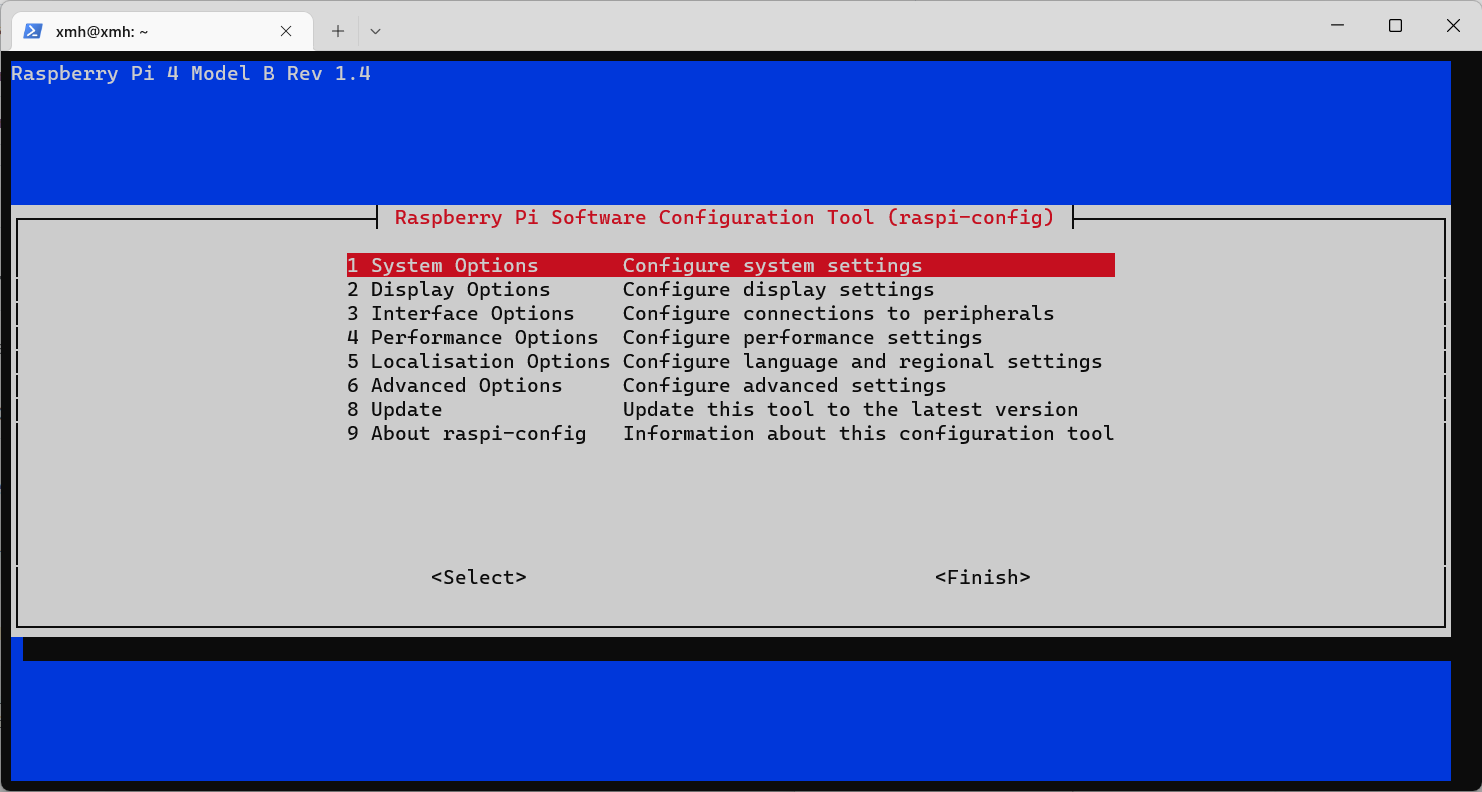
\includegraphics[height=1.5 in]{../pic/PicamEN1.png}}
	\hspace{0 pt}
	\subfigure[Enable the Camera]{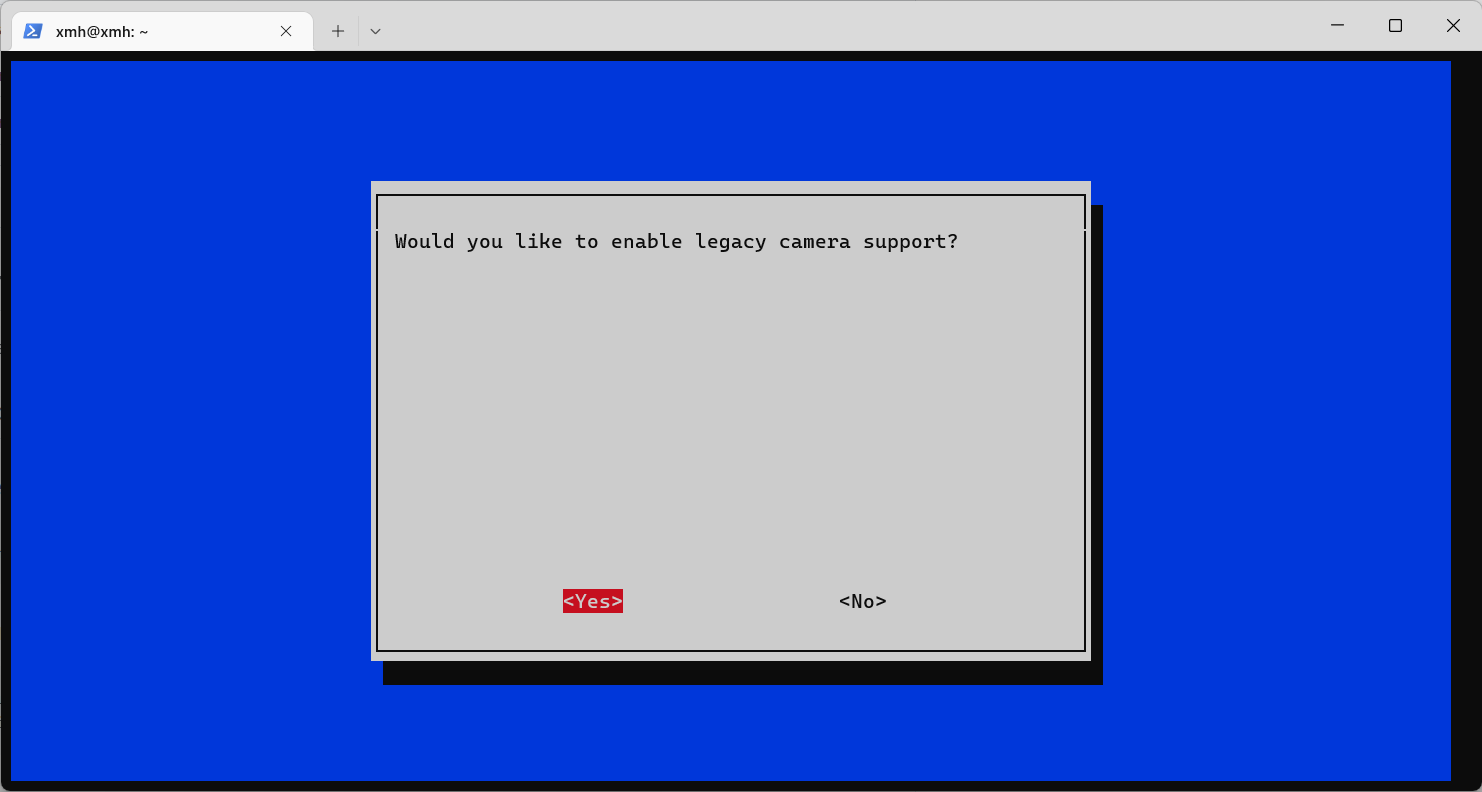
\includegraphics[height=1.5 in]{../pic/PicamEN2.png}}
	\caption{raspi-config}
	\label{fig:PicamEN}
\end{figure}

\section{Implement}

\subsection{Run MJPG-streamer server}

It is not such easy to run a server of MJPG-streamer, so I found a repository in GitHub which has Instructions and helper scripts for running mjpg-streamer on Raspberry Pi\cite{gh:rpi-mjpg-streamer}.

It don't take too much time to implement that. After that I can access the server by browser using the IP mentioned in Section~\ref{sec:basicSetting}, soon I have the \emph{first} photo. See Fig.~\ref{fig:FirstPicOfPicam}.

\begin{figure}[!h]
	\centering
	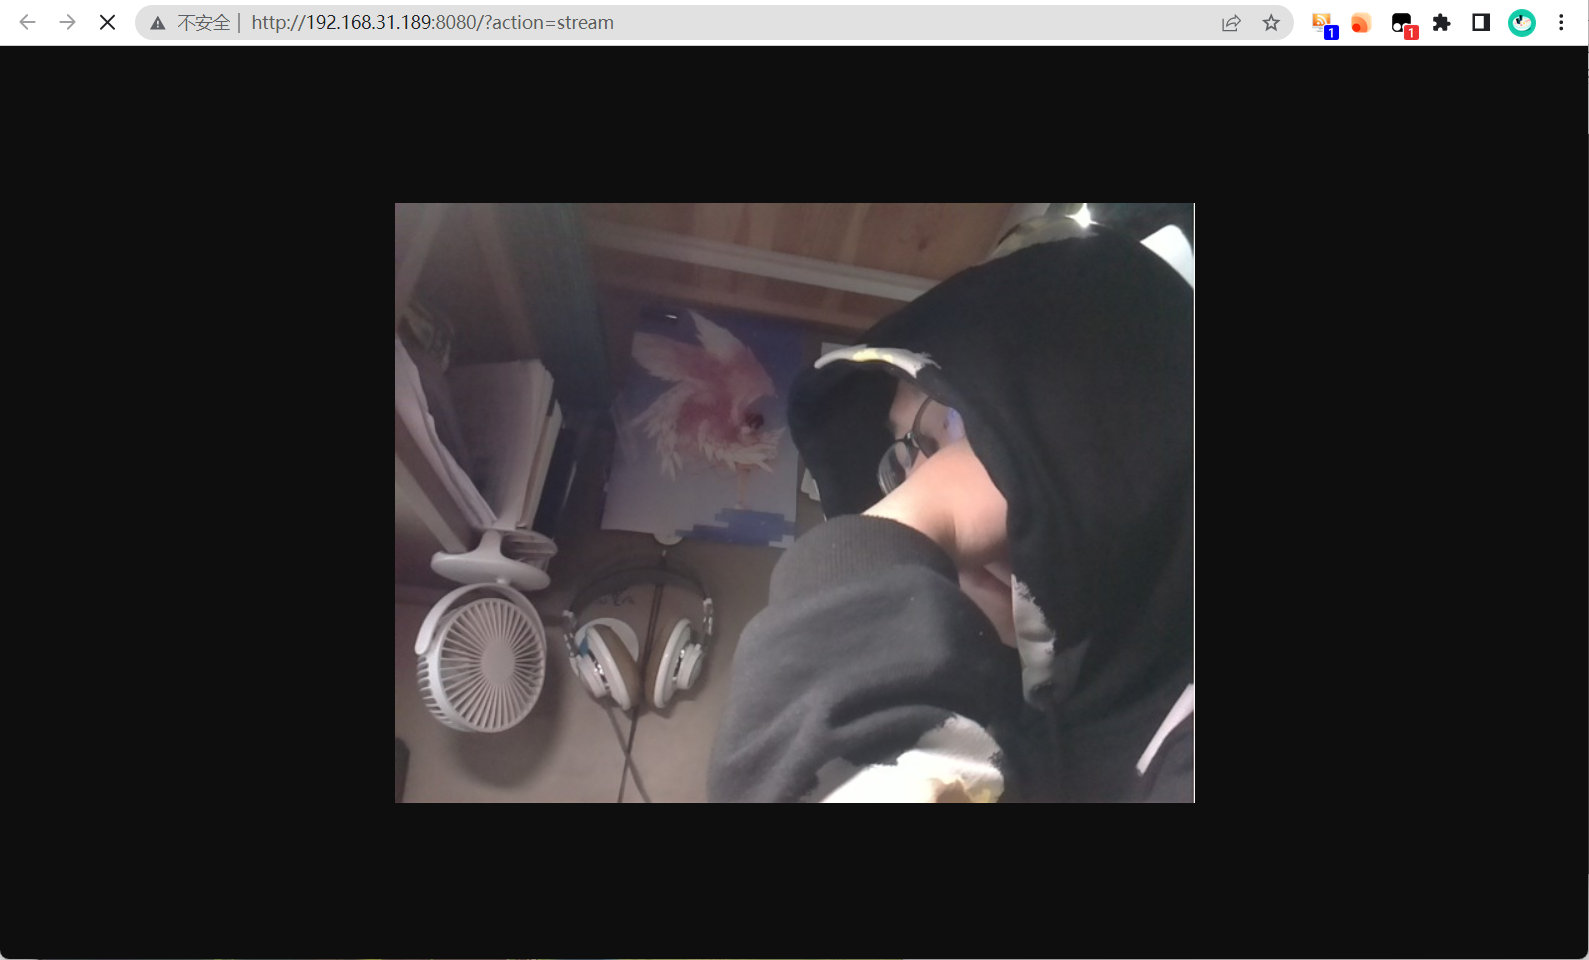
\includegraphics[width=5 in]{../pic/FirstPicOfPicam.png}
	\caption{My First Photo by Pi Camera}
	\label{fig:FirstPicOfPicam}
\end{figure}

\subsection{Broadcast in School}

The next problem is to Mirroring it to the Public Network. At the beginning, I try to use the iLZU to do that. According to my test before, If we can know the local IP we are using to access the iLZU (campus network), 2 devices connected to the iLZU can \emph{find} each other. By referring the webpage \verb|http://10.10.0.166:8800/home|, I knew the local IP is \verb|172.23.xxx.xxx| and it changes in regular basis. I try to ask other students to have a try to access my Raspberry Pi, and it was a big success.

\subsection{Fast Reverse Proxy}

But I still want to access the stream server without connecting the campus network. So, I use fast reverse proxy\cite{gh:frp}. For other reasons, I have a VPS which has its own IPv4. I deployed the server of frp on that machine and release the port 7000 as the proxy port and release the 80 as the service port. And deployed the client side on my Raspberry Pi. I will show my configure files in Code Listing section and that will be more clear.

So, I can now firstly access the 80 port of the VPS and then the VPS relay the data to my Raspberry Pi. See Fig.~\ref{fig:SecondPicOfPicam}

\begin{figure}[!h]
	\centering
	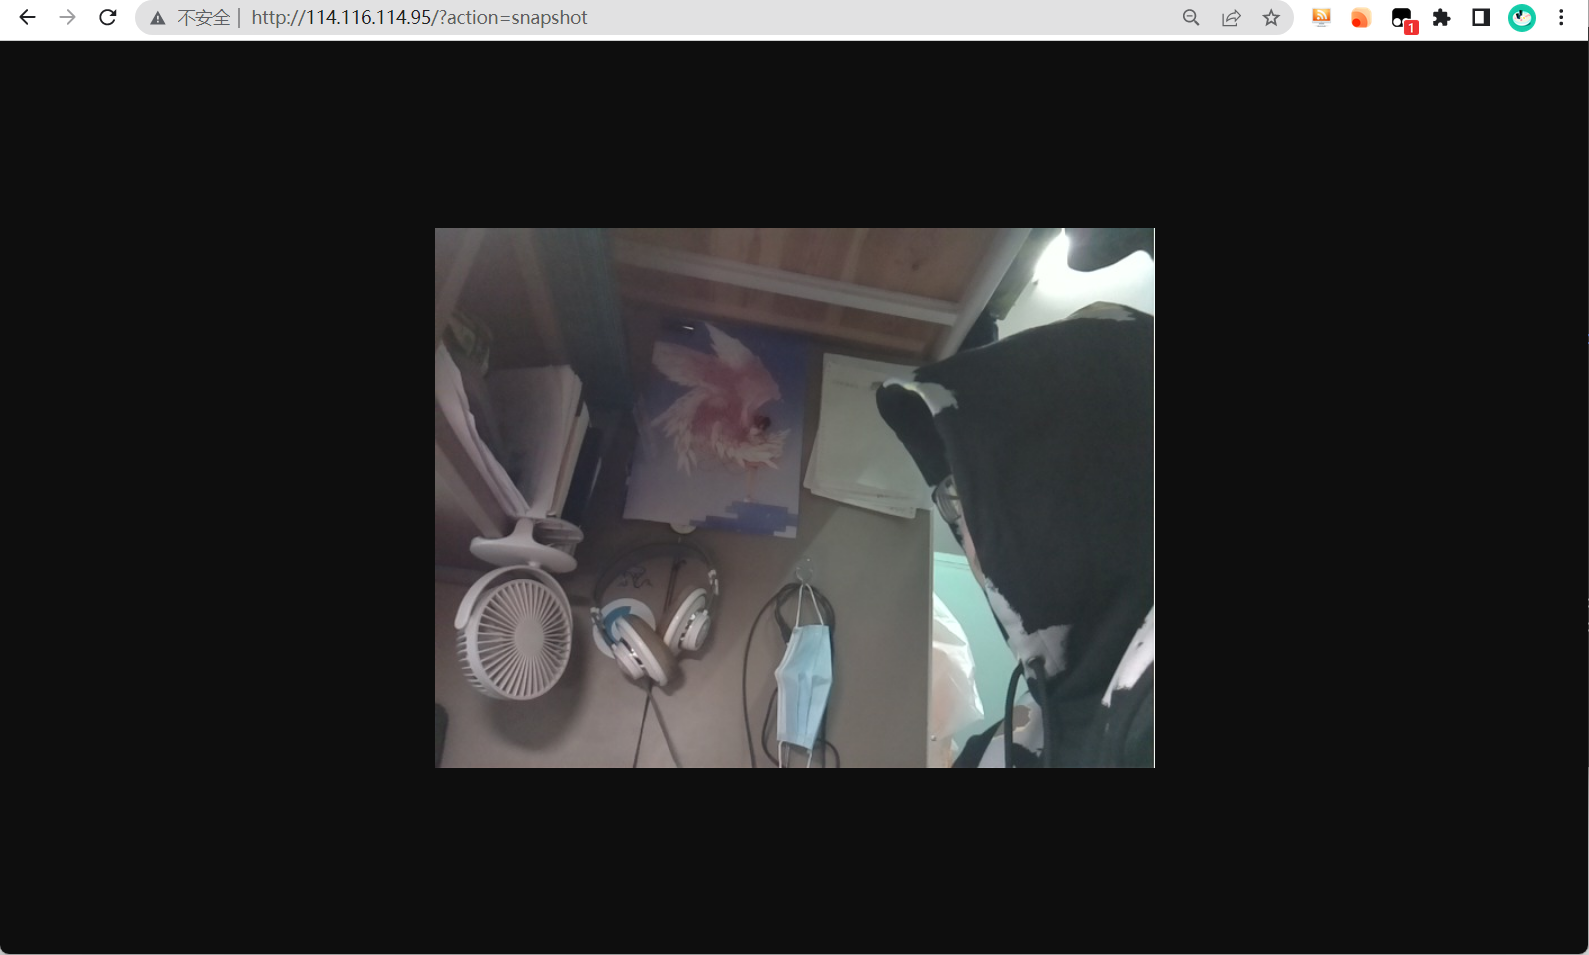
\includegraphics[width=5 in]{../pic/SecondPicOfPicam.png}
	\caption{My Second Photo by Pi Camera}
	\label{fig:SecondPicOfPicam}
\end{figure}

For safety's sake, I want to change the default web application username and password into \verb|xmh| and \verb|xmhxmhxmh|.

\section{Preparation For OpenCV}
The future goal is to server a face-recognition back end, so it is important to use python to control the camera. Then, deploying an environment of OpenCV is what I need to do. 

\verb|sudo apt-get install python3-opencv|

\verb|pip3 install numpy --upgrade|

After installing OpenCV and numpy, I shouldn't forget to install the packets below, otherwise python will tell me to install it.

\verb|sudo apt-get install libatlas-base-dev|

I write the code to let python to control camera and write the image into file. See in the Code Listing section.

\bibliographystyle{ieeetr}
\bibliography{../bib/database}

\begin{appendices}
\section{Code Listing}
\begin{python}
	#use OpenCV to take a photo and save it
	import cv2
	import numpy

	#init
	camera = cv2.VideoCapture(1)

	#read the camera
	ret,img = camera.read()

	#save to snapshot.jpg
	cv2.imwrite('./img.jpg',img)

	#release the camera
	camera.release()
	cv2.destroyAllWindows()
\end{python}
\begin{python}
	#use http request to download the snapshot generated by MJPG-streamer
	import requests

	od = {'action':'snapshot'}

	authe = ('xmh','xmhxmhxmh')

	response = requests.get("http://mc.xwxstudio.com/?",params=od, auth=authe)
	response.raise_for_status()
	with open('./snapshot.jpg','wb') as f:
	    f.write(response.content)
\end{python}
\begin{lstlisting}
	//the configure of frp server
	[common]
	bind_port = 7000
\end{lstlisting}
\begin{lstlisting}
	// the configure of frp client
	[common]
	server_addr = 114.116.114.95
	server_port = 7000

	[webcam]
	type = tcp
	local_ip = 127.0.0.1
	local_port = 8080
	remote_port = 80
\end{lstlisting}
\end{appendices}

\end{document}